\documentclass[../../../main.tex]{subfiles}

\begin{document}
\begin{multicols}{2}[\section{Fundamentals of mathematics}]
    \subsection{Introduction}
    \begin{axiom}[Peano axioms]\hfill
        \begin{enumerate}
            \item $1\in\NN$.
            \item $\forall n\in\NN$, exists a ``successor" $S(n)\in\NN$ of $n$.
            \item $\forall n\in\NN$, $S(n)\ne 1$.
            \item $\forall n,m\in\NN$, $n=m\iff S(n)=S(m)$.
            \item \textit{(Induction axiom)} If $K\subseteq\NN$ is a set such that:
            \begin{enumerate}
                \item $1\in K$.
                \item $\forall k\in K$, $S(k)\in K$.
            \end{enumerate}
            Then, $K=\NN$.
        \end{enumerate}
    \end{axiom}
    \begin{axiom}[Induction axiom]
        Peano's 5th axiom can be stated in the following way: Let $\phi$ be a predicate\footnote{A \textit{predicate} is a formula that can be evaluated to true or false in function of the values of the variables that occur in it.} such that:
        \begin{enumerate}
            \item $\phi(1)$ is true.
            \item $\forall n\in\NN$, $\phi(n)$ being true implies that $\phi(S(n))$ is true.
        \end{enumerate}
        Then, $\phi(n)$ is true for all $n\in\NN$.
    \end{axiom}  
    \begin{prop}
        All non-empty subsets of $\NN$ have a first element.
    \end{prop}
    \begin{prop}
        If a set $A$ satisfies the first four Peano's axioms and has the property that all non-empty subsets it have a first element, then $A$ also satisfies the induction axiom.
    \end{prop}
    \subsection{Set theory}
    \subsubsection*{Definitions and basic operations}
    \begin{definition}
        A \textit{set} is a collection of distinct elements.
    \end{definition}
    \begin{definition}
        Let $A$ be a finite set. The \textit{cardinal of $A$}, $|A|$, is the number of elements in $A$.
    \end{definition}
    \begin{definition}
        Let $A$ be a set. We say a set $B$ is a \textit{subset} of $A$, denoted by $B\subseteq A$, if and only if all elements of $B$ are also elements of $A$
    \end{definition}
    \begin{definition}[Axiom of extensionality]
        Let $A$, $B$ be two sets. We say that $A$ and $B$ are \textit{equal}, $A=B$, if and only if $A\subseteq B$ and $B\subseteq A$.
    \end{definition}
    \begin{definition}
        Let $A$ be set. The subset $\mathcal{P}(A)$, called \textit{power set}, is the set of all subsets of $A$.
    \end{definition}
    \begin{definition}
        We define the \textit{empty set} $\emptyset$ as the unique set having no elements.
    \end{definition}
    \begin{definition}
        Let $A$, $B$ be two sets. The \textit{intersection of $A$ and $B$}, $A\cap B$, is the set of all elements of both $A$ and $B$. That is, $$A\cap B=\{x:x\in A\text{ and }x\in B\}.$$
    \end{definition}
    \begin{prop}
        Let $A$, $B$, $C$ be three sets. Then:
        \begin{enumerate}
            \item $A\cap B=B\cap A$.
            \item $A\cap(B\cap C)=(A\cap B)\cap C$.
            \item $A\cap B\subseteq A$.
            \item $A\cap\emptyset=\emptyset$.
            \item $A\subseteq B\iff A\cap B=B$.
            \item If $C\subseteq A$ and $C\subseteq B$, then $C\subseteq A\cap B$.
        \end{enumerate}
    \end{prop}
    \begin{definition}
        Let $A$, $B$ be two sets. The \textit{union of $A$ and $B$}, $A\cup B$, is the set of all elements of either $A$ or $B$. That is, $$A\cup B=\{x:x\in A\text{ or }x\in B\}.$$
    \end{definition}
    \begin{prop}
        Let $A$, $B$, $C$ be three sets. Then:
        \begin{enumerate}
            \item $A\cup B=B\cup A$.
            \item $A\cup(B\cup C)=(A\cup B)\cup C$.
            \item $A\subseteq A\cup B$.
            \item $A\cup\emptyset=A$.
            \item $A\subseteq B\iff A\cup B=B$.
            \item If $A\subseteq C$ and $B\subseteq C$, then $A\cup B\subseteq C$.
        \end{enumerate}
    \end{prop}
    \begin{prop}
        Let $A$, $B$, $C$ be three sets. Then:
        \begin{enumerate}
            \item $A\cap (B\cup C)=(A\cap B)\cup (A\cap C)$.
            \item $A\cup (B\cap C)=(A\cup B)\cap (A\cup C)$.
        \end{enumerate}
    \end{prop}
    \begin{definition}
        Let $U$ be a set and $A\subseteq U$ be a subset of $U$. The \textit{complement of $A$ in $U$} is the set of elements not in $A$. That is, $$A^c=\{x\in U:x\notin A\}.$$
    \end{definition}
    \begin{prop}[De Morgan's laws]
        Let $U$ be a set and $A$, $B$ be two subsets of $U$. Then:
        \begin{enumerate}
            \item $(A\cup B)^c=A^c\cap B^c$.
            \item $(A\cap B)^c=A^c\cup B^c$.
        \end{enumerate}
    \end{prop}
    \begin{definition}
        Let $U$ be a set and $A$, $B$ be two subsets of $U$. The \textit{set difference of $A$ and $B$}, $A\setminus B$, is the set of elements in $A$ but not in $B$. That is, $$A\setminus B=\{x\in A:x\notin B\}.$$
    \end{definition}
    \begin{prop}
        Let $A$, $B$, $C$ be three sets. Then:
        \begin{enumerate}
            \item $A\setminus B=A\cap B^c$.
            \item $C\setminus(A\cap B)=(C\setminus A)\cup (C\setminus B)$.
            \item $C\setminus(A\cup B)=(C\setminus A)\cap (C\setminus B)$.
        \end{enumerate}
    \end{prop}
    \begin{center}
        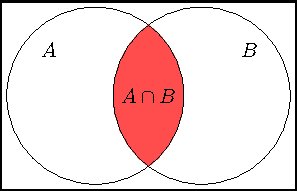
\includegraphics[width=0.49\linewidth]{Images/intersection.tex}\hfill
        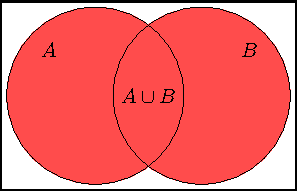
\includegraphics[width=0.49\linewidth]{Images/union.tex}\\
        \vspace{0.02\linewidth}
        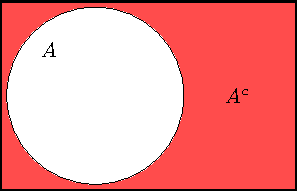
\includegraphics[width=0.49\linewidth]{Images/complement.tex}\hfill
        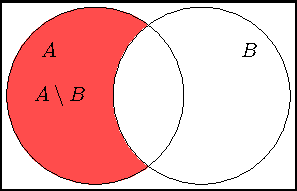
\includegraphics[width=0.49\linewidth]{Images/difference.tex}
        \captionof{figure}{Venn diagrams}
    \end{center}
    \begin{definition}
        Let $A$, $B$ be two sets. The \textit{Cartesian product}, $A\times B$, is the set $$A\times B=\{(a,b): a\in A\text{ and }b\in B\}.$$
    \end{definition}
    \begin{prop}
        Let $A$, $B$, $C$ be three sets. Then:
        \begin{enumerate}
            \item $A\times \emptyset=\emptyset\times A=\emptyset$.
            \item $A\times(B\cap C)=(A\times B)\cap(A\times C)$.
            \item $A\times(B\cup C)=(A\times B)\cup(A\times C)$.
        \end{enumerate}
    \end{prop}
    \subsubsection*{Functions between sets}
    \begin{definition}
        Let $A$, $B$ be two sets. A \textit{function from $A$ to $B$} is a binary relation between $A$ and $B$ that associates to each element of $A$ exactly one element of $B$.
    \end{definition}
    \begin{definition}
        Let $A$, $B$, $C$ be three sets and $f:A\rightarrow B$, $g:B\rightarrow C$ be two functions. The \textit{composition $g\circ f$} is:
        $$\begin{array}{r@{\hspace{0.5\tabcolsep}}c@{\hspace{0.5\tabcolsep}}c@{\hspace{0.5\tabcolsep}}c@{\hspace{0.5\tabcolsep}}c}
            g\circ f:A&\longrightarrow & B & \longrightarrow &C\\
            a&\longmapsto & f(a) & \longmapsto & g[f(a)]
        \end{array}$$
    \end{definition}
    \begin{definition}
        Let $f:A\rightarrow B$ be a function and $U\subseteq A$ be a subset. The \textit{image of $U$} is the subset of $B$ defined by $f(U)=\{f(u): u\in U\}$. If $U=A$, $f(U)=f(A)=:\im f$ is the \textit{image of $f$}.
    \end{definition}
    \begin{definition}
        Let $f:A\rightarrow B$ be a function and $b\in B$. The \textit{preimage of $b$} is the set of elements $a\in A$ such that $f(a)=b$. More generally, if $V\subseteq B$, the \textit{preimage of $V$} is the subset of $A$ defined by: $$f^{-1}(V)=\{a\in A: f(a)=v\in V\}.$$
    \end{definition}
    \begin{prop}
        Let $f:A\rightarrow B$ be a function and $U\subseteq A$ be a subset of $A$. Then,
        \begin{enumerate}
            \item $f\left(\bigcup_{i\in I}U_i\right)\subseteq\bigcup_{i\in I}f(U_i)$.
            \item $f\left(\bigcap_{i\in I}U_i\right)\subseteq\bigcap_{i\in I}f(U_i)$.
            \item $f(U^c)\subseteq f(U)^c$.
        \end{enumerate}
    \end{prop}
    \begin{definition}
        Let $f:A\rightarrow B$ be a function. The following statements are equivalent:
        \begin{enumerate}
            \item $\forall b\in B$, $f^{-1}(b)$ has no more than one element.
            \item $\forall a_1,a_2\in A$, if $a_1\ne a_2$, then $f(a_1)\ne f(a_2)$.
            \item $\forall a_1,a_2\in A$, if $f(a_1)= f(a_2)$, then $a_1=a_2$.
        \end{enumerate}
        If $f$ satisfies one of these conditions, then it satisfies the other two and we say that $f$ is \textit{injective}.
    \end{definition}
    \begin{prop}
        Let $f:A\rightarrow B$, $g:B\rightarrow C$ be two functions.
        \begin{enumerate}
            \item If $f$ and $g$ are injective, then $g\circ f$ is injective.
            \item If $g\circ f$ is injectiva, then $f$ is injective.
        \end{enumerate}
    \end{prop}
    \begin{definition}
        Let $f:A\rightarrow B$ be a function. The following statements are equivalent:
        \begin{enumerate}
            \item The preimage of each element of $B$ has at least one element.
            \item $\forall b\in B$, $\exists a\in A$ such that $f(a)=b$.
            \item $\im f=B$.
        \end{enumerate}
        If $f$ satisfies one of these conditions, then it satisfies the other two and we say that $f$ is \textit{surjective}.
    \end{definition}
    \begin{prop}
        Let $f:A\rightarrow B$, $g:B\rightarrow C$ be two functions.
        \begin{enumerate}
            \item If $f$ and $g$ are surjective, then $g\circ f$ is surjective.
            \item If $g\circ f$ is surjective, then $g$ is surjective.
        \end{enumerate}
    \end{prop}
    \begin{definition}
        Let $f:A\rightarrow B$ be a function. We say that $f$ is \textit{bijective} if it is both injective and surjective. Bijective functions $f^{-1}:B\rightarrow A$.
    \end{definition}
    \begin{prop}
        Let $f:A\rightarrow B$ be a bijective function. The $f$ has an associated inverse function $f^{-1}:B\rightarrow A$ defined as:
        \begin{align*}
            f^{-1}:B&\longrightarrow A\\
            b&\longmapsto f^{-1}(b)
        \end{align*}
    \end{prop}
    \begin{theorem}
        Let $f:A\rightarrow B$ be a function. $f$ is invertible (that is admits and inverse function) if and only if $f$ is bijective.
    \end{theorem}
    \subsection{Logic and propositional calculus}
    \begin{definition}
        Let $P$ be a proposition. Then, $\lnot P$ expresses the \textit{negation of $P$}. 
    \end{definition}
    \begin{definition}
        Let $P$, $Q$ be propositions. Then, $P\land Q$ expresses that \textit{$P$ and $Q$ are both true.}
    \end{definition}
    \begin{definition}
        Let $P$, $Q$ be propositions. Then, $P\lor Q$ expresses that \textit{either $P$ or $Q$ are true}.
    \end{definition}
    \begin{definition}
        Let $P$, $Q$ be propositions. Then, $P\Rightarrow Q$ expresses that \textit{$Q$ is true whenever $P$ is true}. Note that $P\Rightarrow Q=Q\lor\lnot P$.
    \end{definition}
    \begin{definition}
        Let $P$, $Q$ be propositions. Then, $P\Leftrightarrow Q$ expresses that \textit{$P$ and $Q$ have the same truth-value}. Note that $P\Leftrightarrow Q=(P\Rightarrow Q)\land(Q\Rightarrow P)$.
    \end{definition}
    \subsection{Symmetric group}
    \begin{definition}
        Let $n\in\mathbb{N}$. We denote by $S_n$ the set of all the bijections $\{1,2,\ldots,n\}$ to itself. An element of $S_n$ is a permutation of $\{1,\ldots,n\}$.
    \end{definition}
    \begin{prop}
        The pair $(S_n,\circ)$, where 
        \begin{align*}
            \circ:S_n\times S_n&\longrightarrow S_n\\
            (\sigma,\tau)&\longmapsto\sigma\circ\tau
        \end{align*}
        is a group\footnote{See definition \ref{AS-group}.} called \textit{symmetric group}.
    \end{prop}
    \begin{theorem}
        The cardinal of $S_n$ is $n!$.
    \end{theorem}
    \begin{definition}
        Let $\sigma\in S_n$. The set $\{m\in\mathbb{N}:\sigma^m=\text{id}\}$ is non-empty. Hence, it contains a minimal element $\text{ord}(\sigma)$. The integer $\text{ord}(\sigma)$ is called the \textit{order of $\sigma$}.
    \end{definition}
    \begin{definition}
        Let $\sigma\in S_n$. The \textit{support of $\sigma$} is: $$\text{supp}(\sigma)=\{k\in\{1,\ldots,n\}: \sigma(k)\ne k\}.$$
    \end{definition}
    \begin{lemma}
        Let $\sigma\in S_n$. Then:
        \begin{enumerate}
            \item $p\in\text{supp}(\sigma)\implies \sigma(p)\in\text{supp}(\sigma)$.
            \item $\text{supp}(\sigma)=\text{supp}(\sigma^{-1})$.
        \end{enumerate}
    \end{lemma}
    \begin{lemma}
        Let $\sigma,\tau\in S_n$. If $\text{supp}(\sigma)\cap\text{supp}(\tau)=\emptyset$, then $\sigma\circ \tau=\tau\circ \sigma$.
    \end{lemma}
    \begin{definition}
        Let $\sigma\in S_n$ and $k\in\{1,\ldots,n\}$. The \textit{orbit of $k$} is the finite set $\{k,\sigma(k),\sigma^2(k),\ldots\}$.
    \end{definition}
    \begin{theorem}[Orbit structure]
        Let $\sigma\in S_n$ and $\Omega=\{\omega_1,\ldots,\omega_k\}$ be the set of all the orbits of $\sigma$. Then:
        \begin{enumerate}
            \item $\bigcup_{j=1}^k \omega_j=\{1,\ldots,n\}$.
            \item If $\omega_i,\omega_j\in\Omega$ and $\omega_i\cap\omega_j\ne\emptyset$, then $\omega_i=\omega_j$.
            \item All orbits are non-empty.
        \end{enumerate}
    \end{theorem}
    \begin{theorem}[Orbit linear structure]
        Let $\sigma\in S_n$, $\omega$ be one of its orbits and $a\in\omega$. If $k=|\omega|$, then $\omega=\{a,\sigma(a),\ldots,\sigma^{k-1}(a)\}$ and $\sigma^k(a)=a$.
    \end{theorem}
    \begin{definition}
        If $\sigma\in S_n$ has a unique orbit with $k>1$ elements, then we say that $\sigma$ is a \textit{cycle of length $k$}. 
    \end{definition}
    \begin{definition}
        A \textit{transposition} $\tau\in S_n$ is a cycle of length 2.
    \end{definition}
    \begin{theorem}
        Let $\sigma\in S_n$, then $\sigma$ can be written uniquely (except for the order) as a product of cycles with pairwise disjoint supports.
    \end{theorem}
    \begin{corollary}
        Let $\sigma\in S_n$ and $\sigma=\sigma_1\cdots\sigma_\ell$ be its descomposition as product of disjoint cycles. Then, $\text{ord}(\sigma)=\lcm(\sigma_1,\ldots,\sigma_\ell)$.
    \end{corollary}
    \begin{corollary}
        Let $\sigma\in S_n$. Then, $\sigma$ is a product of transpositions.
    \end{corollary}
    \begin{definition}
        Let $\sigma\in S_n$. The \textit{sign of $\sigma$} is $\varepsilon(\sigma)=(-1)^{n-r}$, where $r$ is the number of orbits of $\sigma$.
    \end{definition}
    \begin{theorem}
        Let $\sigma\in S_n$ be a permutation and $\tau\in S_n$ be a transposition. Then, $\varepsilon(\sigma\tau)=\varepsilon(\sigma)\varepsilon(\tau)=-\varepsilon(\sigma)$.
    \end{theorem}
    \begin{corollary}
        Let $\sigma\in S_n$ be such that $\sigma=\tau_1\cdots\tau_\ell$, where $\tau_i\in S_n$ are transpositions for $i=1,\ldots,\ell$. Then, $\varepsilon(\sigma)=(-1)^\ell$.
    \end{corollary}
    \begin{corollary}
        The parity of the number of transpositions in which $\sigma\in S_n$ can be written is invariant.
    \end{corollary}
    \begin{corollary}
        The function
        \begin{align*}
            \varepsilon:S_n&\longrightarrow\{+1,-1\}\\
            \sigma&\longmapsto\varepsilon(\sigma)
        \end{align*}
        is a group morphism\footnote{See definition \ref{AS-groupmorphism}.}.
    \end{corollary}
    \subsection{Equivalence relations and order relations}
    \subsubsection*{Equivalence relations}
    \begin{definition}
        Let $A$ be a set and $\sim$ be a binary relation on $A$. We say that $\sim$ is an \textit{equivalence relation} if and only if the following properties are satisfied:
        \begin{enumerate}
            \item Reflexivity: $$a\sim a,\quad\forall a\in A.$$
            \item Symmetry: $$\text{If }a\sim b, \text{ then }b\sim a,\quad\forall a,b\in A.$$
            \item Transitivity:
            $$\text{If }a\sim b\text{ and }b\sim c,\text{ then }a\sim c,\quad\forall a,b,c\in A.$$
        \end{enumerate}
    \end{definition}
    \begin{definition}
        Let $\sim$ be an equivalence relation on a set $A$ and $a\in A$. The \textit{equivalence class of $a$} under $\sim$ is the subset of $A$: $$[a]=\bar{a}=\{b\in A: a\sim b\}.$$
    \end{definition}
    \begin{theorem}
        Let $\sim$ be an equivalence relation on a set $A$. The equivalence classes $\sim$ form a partition of $A$. That is, if $\{\omega_i\}$ are the equivalence classes, then:
        \begin{enumerate}
            \item $\bigcup_{i\in I} \omega_i=A$.
            \item If $i,j\in I$ and $\omega_i\cap\omega_j\ne\emptyset$, then $\omega_i=\omega_j$.
            \item If $i\in I\implies\omega_i\ne\emptyset$.
        \end{enumerate}
    \end{theorem}
    \begin{definition}
        Let $\sim$ be an equivalence relation on a set $A$. We define the quotient set, $\quot{A}{\!\sim}$, as the set of all equivalence classes of $\sim$.
    \end{definition}
    \subsubsection*{Order relations}
    \begin{definition}
        Let $A$ be a set and $\leq$ be a binary relation on $A$. We say $\leq$ is a \textit{partial order relation} if and only if the following properties are satisfied:
        \begin{enumerate}
            \item Reflexivity:
            $$a\leq a,\quad\forall a\in A.$$
            \item Antisymmetry:
            $$\text{If }a\leq b\text{ and }b\leq a,\text{ then }a=b,\quad\forall a,b\in A.$$
            \item Transitivity:
            $$\text{If }a\leq b\text{ and }b\leq c,\text{ then }a\leq c,\quad\forall a,b,c\in A.$$
        \end{enumerate}
        The pair $(A,\leq)$ is called a \textit{partially ordered set}.
    \end{definition}
    \begin{definition}
        Let $(A,\leq)$ be a partially ordered set. We say that $a\in A$ is a \textit{minimal element} if and only if $b\leq a\implies b=a$, $\forall b\in A$. Futhermore, $a$ is a \textit{least element} if and only if $a\leq b$, $\forall b\in A$. Analogously, we say that $a\in A$ is a \textit{maximal element} if and only if $b\geq a\implies b=a$, $\forall b\in A$. We say that $a\in A$ is a greatest element if and only if $a\geq b$, $\forall b\in A$.
    \end{definition}
    \begin{lemma}
        Let $(A,\leq)$ be a partially ordered set. If $(A,\leq)$ admits a minimum, this is unique. 
    \end{lemma}
    \begin{definition}
        Let $A$ be a set. A \textit{total order relation} on $A$ is a partial order relation in which any two elements of $A$ are comparable. That is, a total order is a binary relation $\leq$ satisfying the properties of a partial order relation and such that $\forall a,b\in A$, we have $a\leq b$ or $b\leq a$.
    \end{definition}
    \begin{definition}
        Let $A$ be a set. A \textit{well-order relation} on $A$ is a total order on $A$ with the property that every non-empty subset of $A$ has a least element. A set $A$ together with a well-order relation is a \textit{well-ordered set}.
    \end{definition}
    \begin{theorem}
        All sets can be well-ordered.
    \end{theorem}
    \subsection{Cardinality and combinatorics}
    \begin{definition}
        Let $A$, $B$ be two sets. We say that $A$ and $B$ have the same cardinal if and only if there exists a bijection $A\rightarrow B$.
    \end{definition}
    \begin{definition}
        Let $A$, $B$ be two sets. We say that $|A|\leq|B|$ if and only if there exists an injection function $A\hookrightarrow B$.
    \end{definition}
    \begin{theorem}[Cantor-Bernstein theorem]
        Let $A$, $B$ be two sets. If there is an injection $A\hookrightarrow B$ and an injection $B\hookrightarrow A$, then there is a bijection $A\rightarrow B$. Comparative of cardinals is an order relation.
    \end{theorem}
    \begin{prop}
        Let $A$, $B$ be two subsets of a set $U$. Then,
        \begin{enumerate}
            \item Inclusion–exclusion principle: $$|A\cup B|=|A|+|B|-|A\cap B|$$
            \item $|A\times B|=|A||B|$
            \item $|A^c|+|A|=|U|$
            \item $|\mathcal{P}(A)|=2^{|A|}$
        \end{enumerate}
    \end{prop}
    \begin{theorem}[Cantor's theorem]
        Let $A$ un set, then $|\mathcal{P}(A)|>|A|$.
    \end{theorem}
    \begin{corollary}
        There is no set containing all sets.
    \end{corollary}
    \begin{corollary}
        There are infinitely many sets with infinite cardinal: $$|\NN|<|\mathcal{P}(\NN)|<|\mathcal{P}(\mathcal{P}(\NN))|<\cdots$$ We denote this cardinals by: $$\aleph_0=|\NN|\quad \aleph_1=|\mathcal{P}(\NN)|\quad \aleph_2=|\mathcal{P}(\mathcal{P}(\NN))|\quad\cdots$$
    \end{corollary}
    \begin{prop}
        Let $A$, $B$ be two finite sets. The set of functions $f:A\rightarrow B$ has cardinal $|B|^{|A|}$.
    \end{prop}
    \begin{definition}
        Let $U$ be a set and $A\in\mathcal{P}(U)$. We define the \textit{characteristic function of $A$} as: 
        \begin{align*}
            \chi_A:U&\longrightarrow\{0,1\}\\
            r&\longmapsto \left\{
            \begin{array}{rcl}
            1 & \text{if} & r\in A \\
            0 & \text{if} & r\notin A
            \end{array}\right.
        \end{align*}
    \end{definition}
    \begin{prop}
        Let $U$ be a set and $A,B\in\mathcal{P}(U)$. Then:
        \begin{enumerate}
            \item $\chi_U=1$
            \item $\chi_{A^c}=1-\chi_A$
            \item $\chi_{A\cap B}=\chi_A\chi_B$
            \item $\chi_{A\cup B}=\chi_A+\chi_B-\chi_A\chi_B$
        \end{enumerate}
    \end{prop}
    \begin{prop}[Binomial coefficient formulas]\hfill
        \begin{enumerate}
            \item $\binom{n}{k}=\frac{n!}{(n-k)!k!}$
            \item $\binom{n}{k}=\binom{n-1}{k}+\binom{n-1}{k-1}$
            \item $\sum_{k=0}^n\binom{n}{k}=2^n$
            \item $k\binom{n}{k}=n\binom{n-1}{k-1}$
            \item $(a+b)^n=\sum_{k=0}^n\binom{n}{k}a^kb^{n-k}$
        \end{enumerate}
    \end{prop}
    \begin{prop}
        Let $f:A\rightarrow B$ be a function between two sets of the same finite cardinal. The following statements are equivalent:
        \begin{enumerate}
            \item $f$ is injective.
            \item $f$ is surjective.
            \item $f$ is bijective.
        \end{enumerate}
    \end{prop}
    \begin{corollary}
        Let $f:A\rightarrow B$ be a function between finite sets. Then:
        \begin{enumerate}
            \item If $f$ is injective, then $|A|\leq|B|$.
            \item If $f$ is surjective, then $|A|\geq|B|$.
        \end{enumerate}
    \end{corollary}
    \begin{theorem}[Pigeonhole principle]
        Let $A$, $B$ be two sets such that $|A|=n$ and $|B|=m$ and $f:A\rightarrow B$ be a function. If $n>m$, then $\exists a,b\in A$ such that $a\ne b$ $f(a)=f(b)$.
    \end{theorem}
    \begin{prop}[Combinations without repetition]
        A combination without repetition is a subset with $m$ elements of a set with $n$ elements. The number of such combinations is $\binom{n}{m}$.
    \end{prop}
    \begin{prop}[Combinations with repetition]
        A combination with repetition is an unordered list with $m$ elements (allowing repetitions) of a set with $n$ elements. The number of such combinations is  $\binom{n+m-1}{m}$.
    \end{prop}
    \begin{prop}[Variations without repetition]
        A variation without repetition is an ordered list of length $m$ elements (without repeating them) taken from a set with $n$ elements. The number of such variations is $\frac{n!}{(n-m)!}$.
    \end{prop}
    \begin{prop}[Variacions with repetition]
        A variation with repetition is an ordered list of length $m$ elements (allowing repetitions) taken from a set with $n$ elements. The number of such variations is $n^m$.
    \end{prop}
    \subsection{Arithmetic}
    \subsubsection*{Integer numbers}
    For some basic definitions in group and ring theory you might need to refer to sections \ref{AS-G} and \ref{AS-R}.
    \begin{definition}
        Let $a,b\in\mathbb{Z}$. We say that \textit{$a$ is a multiple of $b$} if there exists $c\in\mathbb{Z}$ such that $a=cb$.
    \end{definition}
    \begin{theorem}
        Let $D,d\in\mathbb{Z}$, $d\ne 0$. Then, there are unique $q,r\in\mathbb{Z}$ such that $D=qd+r$ and $0\leq r\leq|d|$.
    \end{theorem}
    \begin{prop}
        Let $a,b\in \mathbb{Z}$. $a\mathbb{Z}\subseteq b\mathbb{Z}\iff b\mid a$.
    \end{prop}
    \begin{corollary}
        Let $a,b\in \mathbb{Z}$. $a\mathbb{Z}=b\mathbb{Z}\iff a=\pm b$.
    \end{corollary}
    \begin{prop}
        Let $a\mathbb{Z}$, $b\mathbb{Z}$ be two ideals of $\ZZ$. Then, $\exists!m\in\mathbb{N}$ such that $a\mathbb{Z}\cap b\mathbb{Z}=m\mathbb{Z}$. This integer $m$ is called the \textit{least common multiple of $a$ and $b$}.
    \end{prop}
    \begin{prop}
        Let $a\mathbb{Z}$, $b\mathbb{Z}$ be two ideals of $\ZZ$. Then, $\exists!d\in\mathbb{N}^*$ such that $a\mathbb{Z}+b\mathbb{Z}=d\mathbb{Z}$. This integer $d$ is called the \textit{greatest common divisor of $a$ and $b$}.
    \end{prop}
    \begin{prop}
        Let $a,b,m,d\in\ZZ$.
        \begin{enumerate}
            \item If $a\mid m$ and $b\mid m$, then $\lcm(a,b)\mid m$.
            \item If $d\mid a$ and $d\mid b$, then $d\mid\gcd(a,b)$.
        \end{enumerate}
    \end{prop}
    \begin{definition}
        Let $a,b\in\mathbb{Z}$. We say that $a$ and $b$ are \textit{coprime} or \textit{relatively prime} if and only if $\gcd(a,b)=1$.
    \end{definition}
    \begin{definition}
        We say that $p\in\ZZ$ is \textit{prime} if and only if $p\mathbb{Z}$ is a maximal ideal. The set of prime numbers is denoted by $\mathbb{P}$.
    \end{definition}
    \begin{prop}
        Let $a\in\ZZ$. Then, $a\in\mathbb{P}$ if and only if $a$ has exactly 4 divisors: $a$, $-a$, 1 and $-1$.
    \end{prop}
    \begin{lemma}
        Let $a,b,k\in\mathbb{Z}$ such that $a\geq b>0$. Then, common divisors of $a$ and $b$ are the same as common divisors of $a+kb$ and $b$.
    \end{lemma}
    \begin{theorem}[Bézout's theorem]
        Let $a,b\in\mathbb{Z}$, then there exists $u,v\in\mathbb{Z}$ such that $au+bv=\gcd(a,b)$. Moreover, $\gcd(a,b)=1\iff\exists u,v\in\mathbb{Z}$ such that $au+bv=1$.
    \end{theorem}
    \begin{theorem}[Gau\ss' theorem]
        Let $a,b\in\mathbb{Z}$. If $a\mid bc$ and $\gcd(a,b)=1$ then $a\mid c$.
    \end{theorem}
    \begin{corollary}
        Let $a,b,c\in\mathbb{Z}$ be integers such that $a$ and $b$ are relatively prime. If $a\mid c$ and $b\mid c$, then $ab\mid c$.
    \end{corollary}
    \begin{theorem}[Prime number theorem]
        Let $x\in\mathbb{R}$. If $\pi(x)$ is the number of prime number less than or equal to $x$, then $\pi(x)\sim\frac{x}{\log(x)}$.
    \end{theorem}
    \begin{theorem}
        Let $a,b\in\mathbb{Z}$. Then, $$\gcd(a,b)\lcm(a,b)=|ab|.$$
    \end{theorem}
    \begin{lemma}
        Let $p\in\mathbb{P}$ and $a\in\mathbb{Z}$. Then, $p\mid a$ or $\gcd(a,p)=1$.
    \end{lemma}
    \begin{corollary}
        Let $a,b\in\ZZ$ and $p\in\mathbb{P}$. If $p\mid ab$, then $p\mid a$ or $p\mid b$.
    \end{corollary}
    \begin{corollary}
        Let $p,q\in\mathbb{P}$. If $p\mid q$, then $p=\pm q$.
    \end{corollary}
    \begin{theorem}[Fundamental theorem of arithmetic]
        Let $n\in\mathbb{N}$ such that $n>1$. Then, $n$ can be represented uniquely (except for the order) as the product of prime numbers.
    \end{theorem}
    \begin{theorem}[Euclid's theorem]
        The set $\mathbb{P}$ is infinite. 
    \end{theorem}
    \begin{theorem}
        Let $a,b,c,x,y\in\ZZ$. The equation $ax+by=c$ has at least a solution if and only if $\gcd(a,b)\mid c$. In this case, if $d=\gcd(a,b)$, $a=a'd$ and $b=b'd$, the set $\mathcal{S}$ of solutions of the equation $ax+by=c$ is $$S=\{(x_0,y_0)+\lambda(-b',a'):\lambda\in\ZZ\},$$ where $(x_0,y_0)$ is a particular solution of the equation. 
    \end{theorem}
    \subsubsection*{Modular arithmetic}
    \begin{definition}
        Let $n,x,y\in\ZZ$. We say $x\sim y\iff x-y\in n\mathbb{Z}$. A commonly used notation for this is $x\equiv y\mod n$. The set of equivalence classes under $\sim$ is denoted by $\quot{\mathbb{Z}}{n\mathbb{Z}}$ and its elements are denoted by $\bar{x}$.
    \end{definition}
    \begin{lemma}
        $\quot{\ZZ}{n\ZZ}$ té $n$ elements.
    \end{lemma}
    \begin{prop}
        Addition and multiplication are well-defined in $\quot{\ZZ}{n\ZZ}$ if we do it in the following way:
        \begin{align*}
            +:\quot{\ZZ}{n\ZZ}\times\quot{\ZZ}{n\ZZ}&\longrightarrow\quot{\ZZ}{n\ZZ}&\cdot:\quot{\ZZ}{n\ZZ}\times\quot{\ZZ}{n\ZZ}&\longrightarrow\quot{\ZZ}{n\ZZ}\\
            (\bar{a},\bar{b})&\longmapsto\overline{a+b}&(\bar{a},\bar{b})&\longmapsto\overline{a\cdot b}
        \end{align*}
    \end{prop}
    \begin{theorem}
        Since $(\mathbb{Z},+,\cdot)$ is a ring, $(\quot{\ZZ}{n\ZZ},+,\cdot)$ is a ring and the projection 
        \begin{align*}
            f:\mathbb{Z}&\longrightarrow\quot{\ZZ}{n\ZZ}\\
            a&\longmapsto\bar{a}
        \end{align*}
        is a ring morphism.
    \end{theorem}
    \begin{lemma}
        Let $n\in\mathbb{Z}$. Then, $\bar{a}\in\quot{\ZZ}{n\ZZ}$ is invertible per a la multiplicació if and only if $\gcd(a,n)=1$.
    \end{lemma}
    \begin{corollary}
        $(\quot{\ZZ}{n\ZZ},+,\cdot)$ is a field if and only if $n\in\mathbb{P}$.
    \end{corollary}
    \begin{theorem}[Chinese remainder theorem]
        Let $m,n\in\ZZ$ be relatively prime. Then, the function
        \begin{align*}
            \psi:\quot{\ZZ}{nm\ZZ}&\longrightarrow\quot{\ZZ}{m\ZZ}\times\quot{\ZZ}{n\ZZ}\\
            \overline{a}^{\scriptscriptstyle mn}&\longmapsto(\overline{a}^{\scriptscriptstyle m},\overline{a}^{\scriptscriptstyle n})
        \end{align*}
        is ring isomorphism.
    \end{theorem}
    \begin{definition}[Euler's totient function]
        Let $n\in\mathbb{N}$. We define the function $\varphi:\NN\rightarrow\NN$ as: 
        \begin{multline*}
            \varphi(n)=|\{\textstyle\alpha\in\quot{\ZZ}{n\ZZ}:\alpha \text{ is invertible}\}|=\\=|\{0<r\leq n: \gcd(r,n)=1\}|.
        \end{multline*}
    \end{definition}
    \begin{lemma}
        Let $m,n\in\ZZ$ be relatively prime. Then, $\varphi(m\cdot n)=\varphi(m)\cdot\varphi(n).$
    \end{lemma}
    \begin{theorem}[Euler's theorem]
        Let $a\in\mathbb{Z}$ and $n\in\mathbb{N}$ such that $\gcd(a,n)=1$, then $$a^{\varphi(n)}\equiv 1\mod n.$$ In particular, $a^{-1}\equiv a^{\varphi(n)-1}\mod n$.
    \end{theorem}
    \begin{theorem}[Fermat's little theorem]
        Let $p\in\mathbb{P}$. Then, $\varphi(p)=p-1$ and $$a^p\equiv a\mod p.$$ In particular, if $\gcd(a,p)=1$, $a^{p-1}\equiv 1\mod p$.
    \end{theorem}
    \subsection{Polynomials}
    \begin{definition}
        Let $R$ be a ring. A \textit{polynomial $p$ with coefficients in $R$} is an expression of the form $$p=p(x)=a_0+a_1x+\cdots+a_nx^n,$$ where $x$ is a \textit{variable} or an \textit{indeterminate} and $a_i\in R$ are the \textit{coefficients}. The term $a_0$ is called \textit{constant term}, and the term $a_n$, \textit{leading coefficient}. Fianlly, the set of all polynomials in the variable $x$ and coefficients in $R$ is denoted by $R[x]$.
    \end{definition}
    \begin{definition}
        Let $p(x)=\sum_{i=0}^na_ix^i\in R[x]$ be a polynomial such that $a_n\ne 0$. Then, we define the \textit{degree of $p(x)$} as $\deg p(x)=n$\footnote{To see properties relating degrees of polynomials see proposition \ref{AG-deg}.}.
    \end{definition}
    \begin{definition}
        Let $p(x),q(x)\in R[x]$ such that $p(x)=\sum_{i=0}^na_ix^i\in R[x]$ and $q(x)=\sum_{i=0}^nn_ix^i\in R[x]$. We define the \textit{sum of $p(x)$ and $q(x)$} as: $$p(x)+q(x)=\sum_{i=0}^n(a_i+b_i)x^i.$$
        We define the \textit{product of $p(x)$ and $q(x)$} as: $$p(x)\cdot q(x)=\sum_{i=0}^nc_ix^i,\quad c_i=\sum_{j=0}^ia_ib_{j-i}.$$
    \end{definition}
    \begin{prop}
        Let $K$ be a field. If $p(x),q(x)\in K[x]$ and $p(x),q(x)\ne 0$, then $p(x)\cdot q(x)\ne 0$.
    \end{prop}
    \begin{theorem}[Euclidian division]
        Let $K$ be a field. Let $p(x),s(x)\in K[x]$ with $s(x)\ne 0$. Then, $\exists! q(x),r(x)\in K[x]$ such that $p(x)=q(x)\cdot s(x)+r(x)$ and $0\leq\deg(r(x))<\deg(s(x))$.
    \end{theorem}
    \begin{theorem}
        Let $K$ be a field. Then, $K[x]$ is a principal ideal, that is, if $I\subset K[x]$ is an ideal, then $\exists p(x)\in K[x]$ such that $I=p(x)\cdot K[x]$.
    \end{theorem}
    \begin{definition}
        Let $K$ be a field. Let $p(x),q(x)\in K[x]$. Then, $\gcd(p(x),q(x))$ is a generator of the ideal $p(x)\cdot K[x]+q(x)\cdot K[x]$ and $\lcm(p(x),q(x))$ is a generator of the ideal $p(x)\cdot K[x]\cap q(x)\cdot K[x]$.
    \end{definition}
    \begin{definition}
        We say that a polynomial $p(x)=\sum_{i=0}^na_ix^i$ is \textit{monic} if $a_n=1$.
    \end{definition}
    \begin{theorem}[Bézout's theorem]
        Let $K$ be a field and $p(x),q(x)\in K[x]$. Then, $\exists u(x), v(x)\in K[x]$ such that $p(x)\cdot u(x)+q(x)\cdot v(x)=\gcd(p(x),q(x))$.
    \end{theorem}
    \begin{definition}
        Two polynomials $p(x)$, $q(x)$ are \textit{coprime} or \textit{relatively prime} if and only if $\gcd(p(x),q(x))=1$.
    \end{definition}
    \begin{theorem}[Gau\ss' theorem]
        Let $K$ be a field and $p(x),a(x),b(x)\in K[x]$. If $p(x)\mid a(x)\cdot b(x)$ and $\gcd(a(x),p(x))=1$, then $p(x)\mid b(x)$.
    \end{theorem}
    \begin{definition}
        Let $K$ be a field. A polynomial $p(x)\in K[x]$ is \textit{prime} if and only if its ideal $p(x)\cdot K[x]$ is maximal, that is, for all ideals $I\subseteq K[x]$ if $p(x)\cdot K[x] \subset I$, then $I=K[x]$.
    \end{definition}
    \begin{definition}
        Let $K$ be a field and $a\in K$. The \textit{evaluation in $a$} is a function $\phi_a$ defined as:
        \begin{align*}
            \phi_a:K[x]&\longrightarrow K\\
            p(x)&\longmapsto p(a)
        \end{align*}
    \end{definition}
    \begin{definition}
        Let $K$ be a field and $a\in K$. $a$ is a \textit{root of $p(x)$} if and only if $\phi_a(p(x))=p(a)=0$.
    \end{definition}
    \begin{theorem}[Ruffini's rule]
        Let $K$ be a field, $p(x)\in K[x]$ and $a\in K$. Then, $x-a\mid p(x)\iff p(a)=0$.
    \end{theorem}
    \begin{definition}
        Let $K$ be a field and $p(x)\in K[x]$. Then, $p(x)$ is \textit{irreducible} if and only if $p(x)\cdot K[x]$ is maximal.
    \end{definition}
    \begin{theorem}
        Let $K$ be a field and $p(x)\in K[x]$. Then, $p(x)$ has at most $\deg(p(x))$ arrels.
    \end{theorem}
    \begin{theorem}[D'Alembert theorem]
        All non-constant polynomials $p(x)\in\mathbb{C}[x]$ has exactly $\deg(p(x))$ roots.
    \end{theorem}
    \begin{corollary}
        Let $p(x)\in\mathbb{C}[x]$ be such that $\deg(p(x))>1$. Then, $\exists!\alpha,r_1,\ldots,r_n\in\mathbb{C}$ such that $$p(x)=\alpha(x-r_1)\cdots(x-r_n),$$ where $r_i$ are the roots of $p(x)$ and $\alpha$ is the leading coefficient of $p(x)$.
    \end{corollary}
    \begin{corollary}
        Let $p(x)\in\mathbb{C}[x]$. The roots of $p(x)$ in $\mathbb{C}\setminus\mathbb{R}$ come in pairs $(r,\overline{r})$, where $\overline{r}$ is the romplex conjugate of $r$.
    \end{corollary}
    \begin{theorem}
        In $\mathbb{R}[x]$ irreducible polynomials are of degree 1 or degree 2.
    \end{theorem}
\end{multicols}
\end{document}